\documentclass{beamer}
\usepackage[utf8]{inputenc}

\usetheme{Madrid}
\usecolortheme{default}
\usepackage{siunitx}


%------------------------------------------------------------
%This block of code defines the information to appear in the
%Title page
\title[Ecommerce-affecting-brickandmortar-retail] %optional
{Transforming in the Digital Tide: An In-depth Analysis of the Impact of E-Commerce on Brick-and-Mortar Retail in China, 2019-2023}


\author{Qingyue Chen 22-737-639\\Shiyang Jin 22-737-712\\
Yuru Jin 21-749-650\\Zhengyu Duan 22-736-904}


\date[11-12-2023] % (optional)
{December 2023}



%End of title page configuration block
%------------------------------------------------------------



%------------------------------------------------------------
%The next block of commands puts the table of contents at the 
%beginning of each section and highlights the current section:

\AtBeginSection[]
{
  \begin{frame}
    \frametitle{Table of Contents}
    \tableofcontents[currentsection]
  \end{frame}
}
%------------------------------------------------------------


\begin{document}

%The next statement creates the title page.
\frame{\titlepage}




\section{Background}

%---------------------------------------------------------
%Changing visivility of the text


\begin{frame}{Background}
  \begin{itemize}
    \item \textbf{Significant Change}: E-commerce reshapes China's retail landscape.
    \item \textbf{Focus}: Analyzing how e-commerce transforms traditional retail.
    \item \textbf{Analysis}: Examining retail trends, online/offline sales, consumer shifts.
    \item \textbf{Goal}: Detailed, data-driven insights into China's evolving retail sector.
    \item \textbf{China's E-commerce Boom}: From RMB 930 billion (2004) to RMB 29,160 billion (2017); 533 million online shoppers by 2017.
    \item \textbf{Global Dominance}: China's global e-commerce market share soared from under 1\% to over 40\%.
  \end{itemize}
\end{frame}

\section{Process}
\begin{frame}{Process}
  \textbf{Assumption:} 
  \begin{itemize}
    \item Data Reliability, Consumer Behavior, Representation, Technology Access, Retail Segmentation.
  \end{itemize}

  \textbf{Predictions:}
  \begin{itemize}
    \item Market Shift: Growing negative correlation between online and offline retail indicates a shift towards digital platforms.
    \item COVID-19 Impact: Pandemic accelerates e-commerce adoption, altering consumer behavior.
  \end{itemize}

  \textbf{Data Section Overview:}
  \begin{itemize}
    \item \textbf{Data Sources:} Primary data from the National Bureau of Statistics of China.
    \item \textbf{Collection Method:} Efficient data gathering using Python-based web scraping tools.
    \item \textbf{Dataset Insights:} Interplay and trends between online and offline retail channels.
  \end{itemize}
\end{frame}

\begin{frame}{Process-Data}
  \textbf{Data Processing Overview:}
  \begin{itemize}
    \item Integration and Summarization: Unifying various datasets.
    \item Handling Data Shortages: Averaging technique for January data.
    \item Correlation Analysis: Examining online-offline sales relationship.
  \end{itemize}

  \textbf{Data Crawling with Python:}
  \begin{itemize}
    \item Data Extraction: HTTP POST requests for retail data.
    \item Parsing and Cleaning: Custom functions for JSON parsing.
    \item Data Structuring: Organizing data in pandas DataFrames.
  \end{itemize}

  \textbf{Key Considerations in Data Handling:}
  \begin{itemize}
    \item Integration of Diverse Data Sources.
    \item Addressing Seasonal Data Shortages.
    \item Ensuring Cumulative Data Accuracy.
    \item Assessing COVID-19's Retail Impact.
  \end{itemize}
\end{frame}



  
\section{Analysis}
\begin{frame}{Descriptive Analysis}

\frametitle{Descriptive Analysis of Retail Sales}

\textbf{Online Sales Trends:}
\begin{itemize}
    \item Monthly sales fluctuate with seasonal peaks.
    \item An increasing trend observed from 2019 to 2023.
    \item Data suggests potential seasonal patterns.
\end{itemize}
\begin{figure}
    \centering
    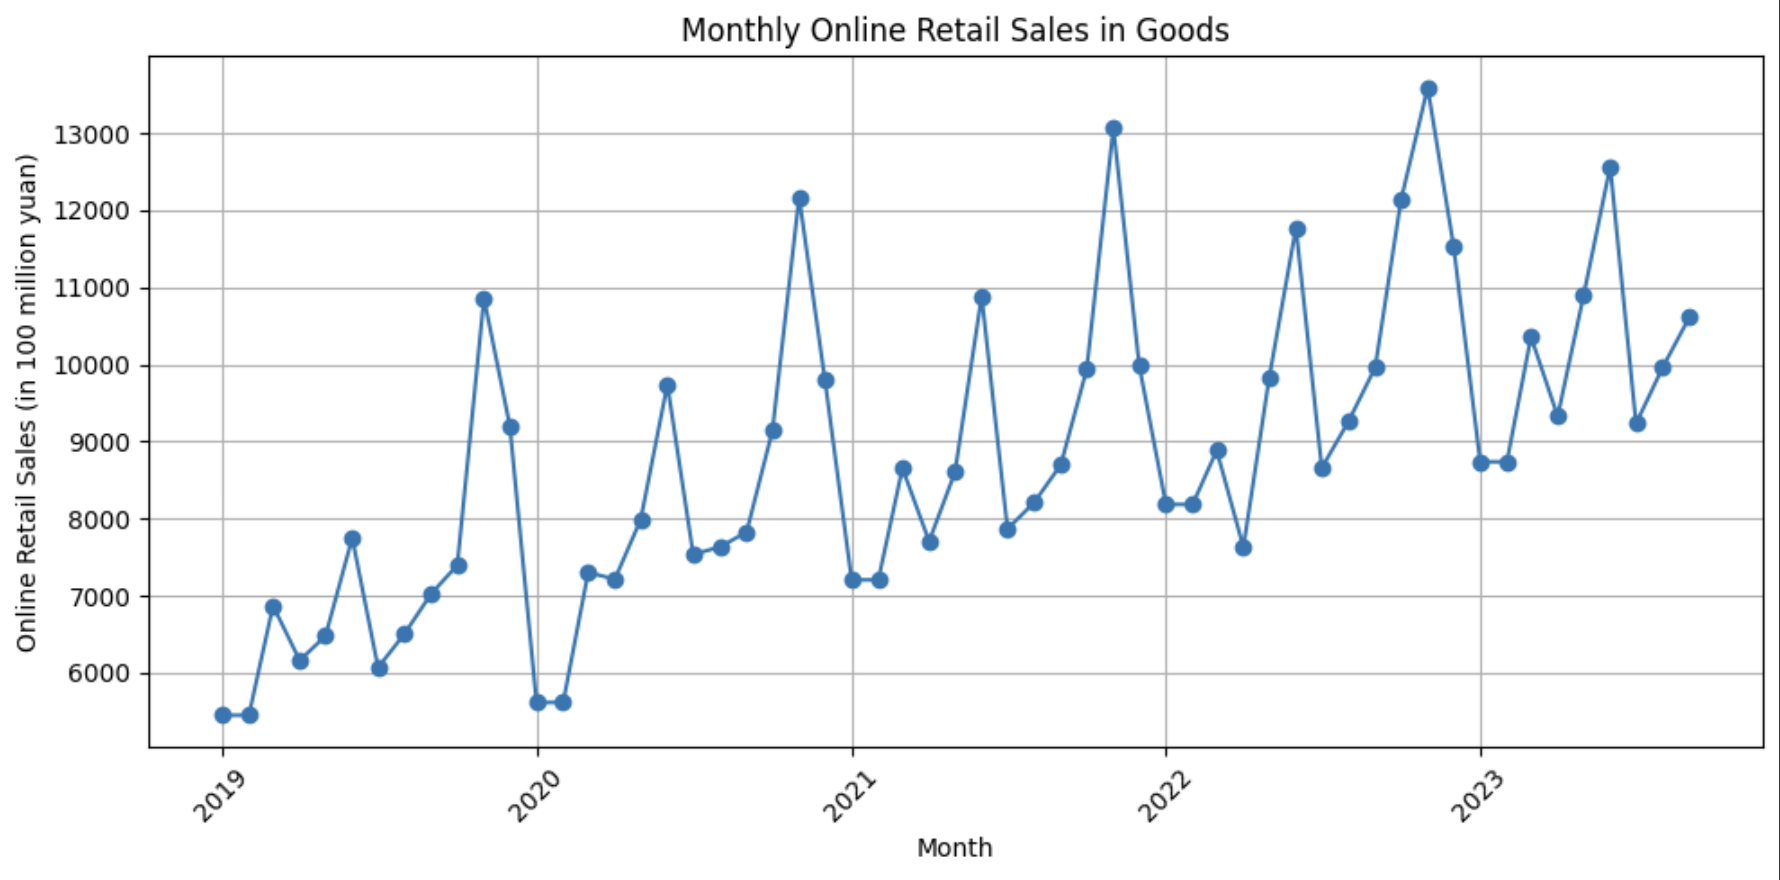
\includegraphics[width=0.75\textwidth]{online_sales_data.png}
    \caption{Monthly Online Sales Data}
\end{figure}
\end{frame}


\textbf{In-Store Sales Patterns:}
\begin{itemize}
    \item Larger fluctuations in sales compared to online.
    \item Sharp increase at the start of 2020, hinting at a possible event impact or seasonal trend.
    \item Trends assist in comparing online vs. in-store performance and strategic planning.
\end{itemize}
\begin{figure}
    \centering
    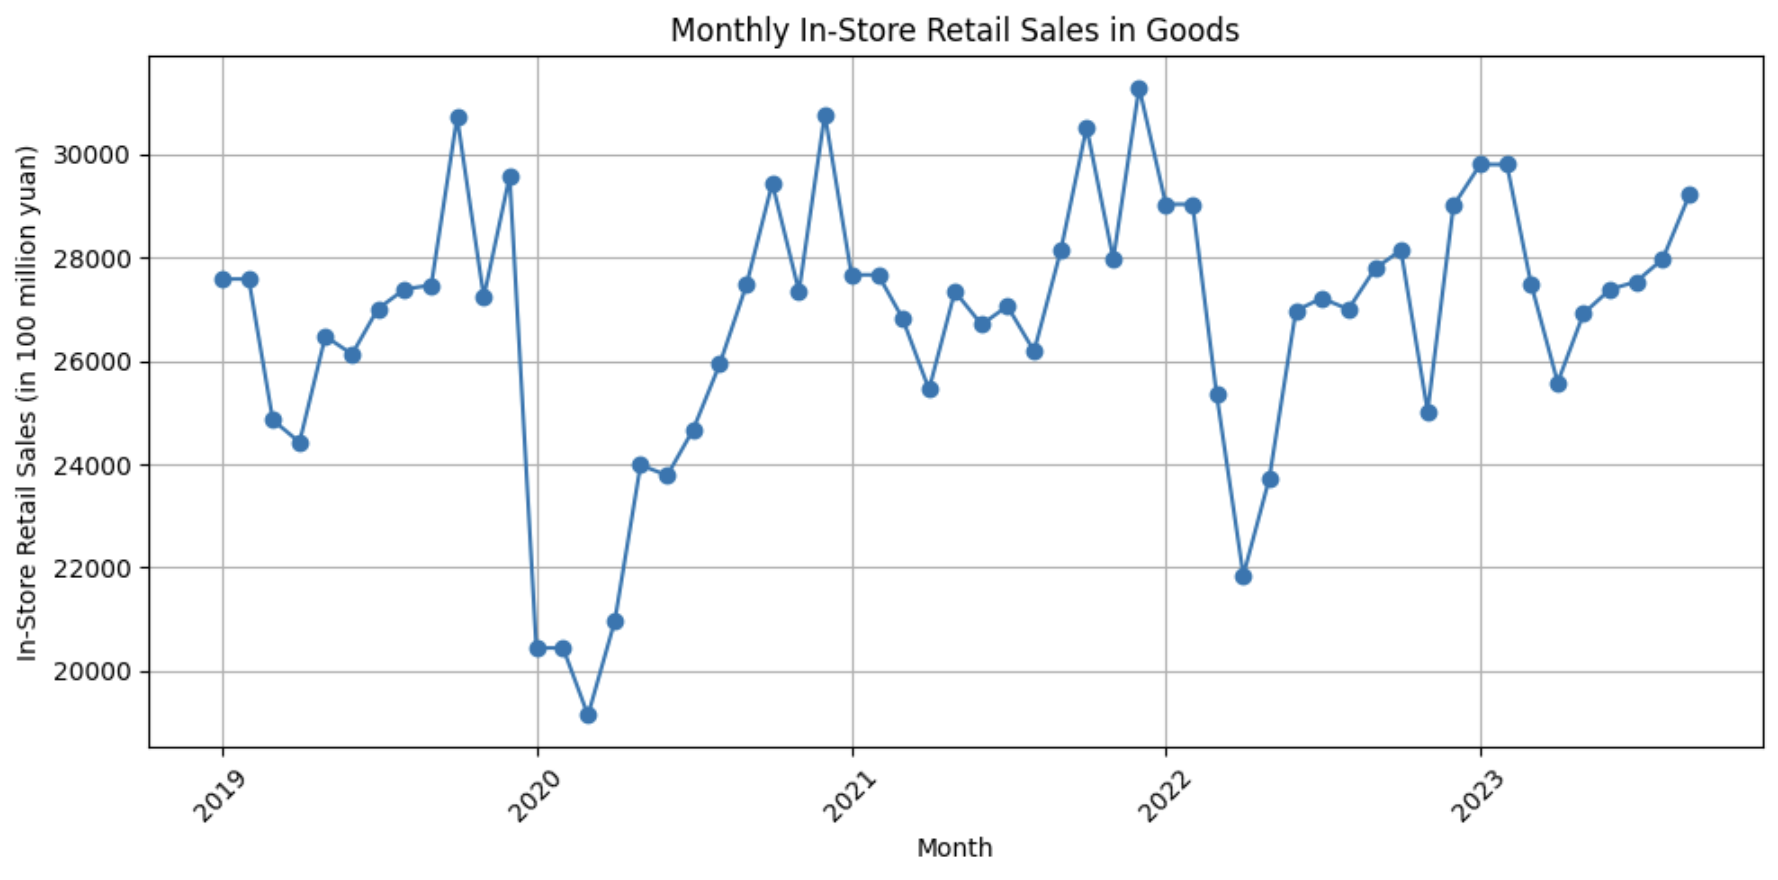
\includegraphics[width=0.75\textwidth]{offline_sales_data.png}
    \caption{Monthly Offline Sales Data}
\end{figure}

\textbf{Trends in In-Store vs. Online Retail Sales:}
\begin{itemize}
    \item Online sales are steadily increasing over time.
    \item In-store sales are more volatile and slightly declining.
    \item The gap between in-store and online sales is narrowing.
\end{itemize}

\begin{figure}
    \centering
    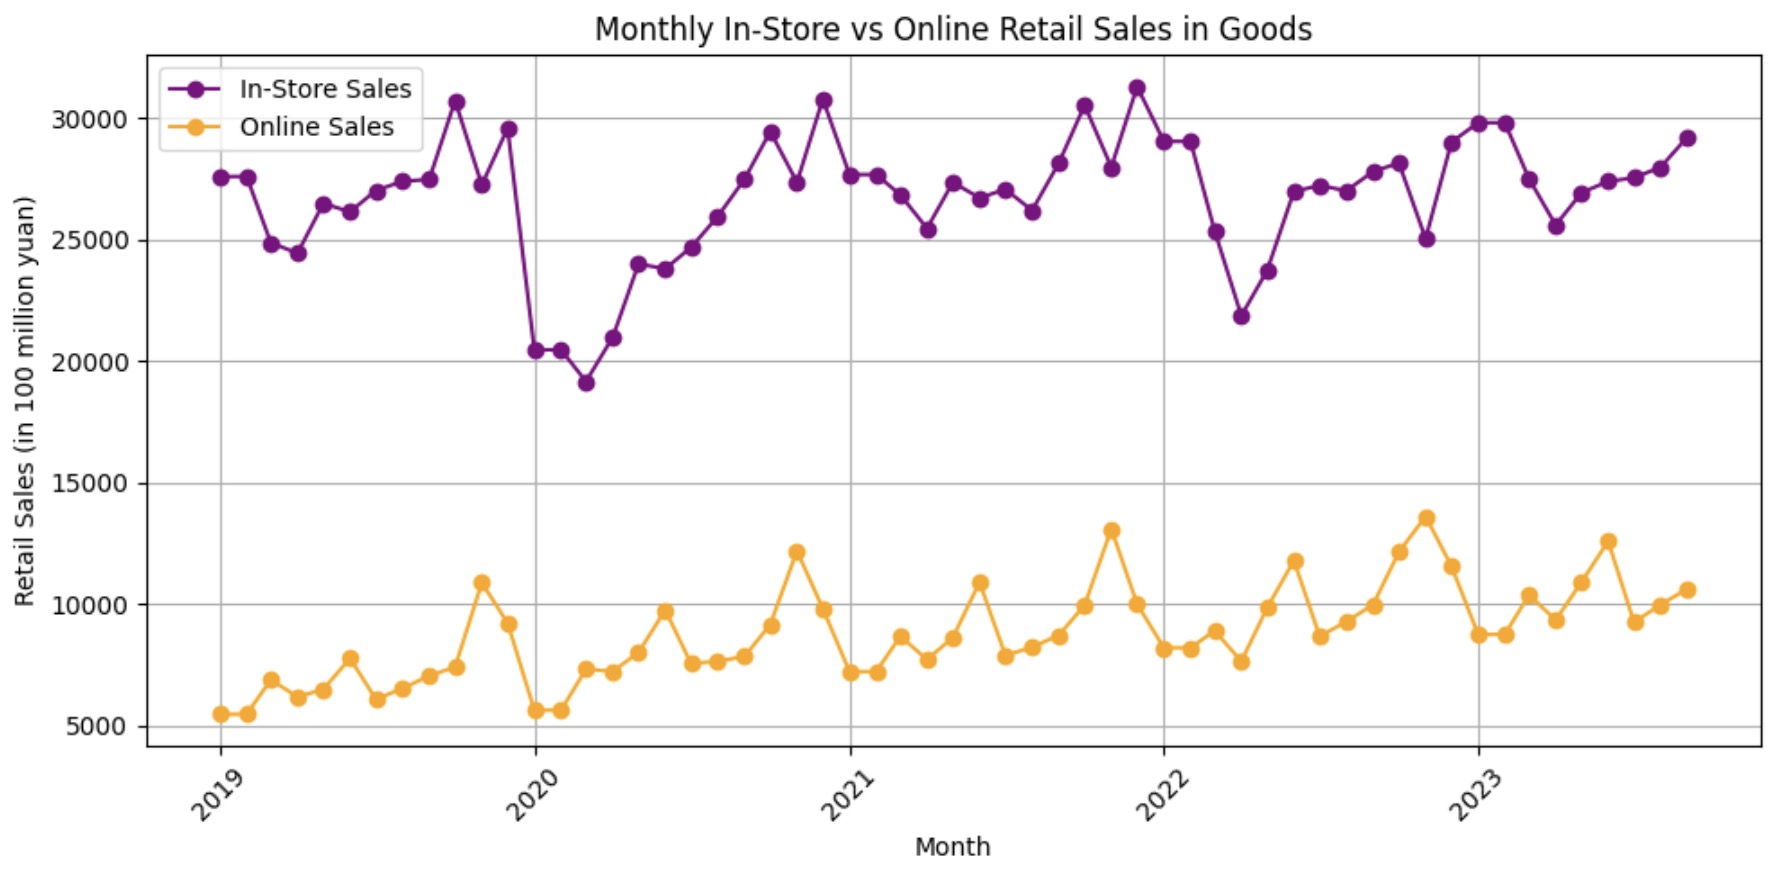
\includegraphics[width=0.75\textwidth]{online_instore_compare.jpg}
    \caption{Online and offline sales compare}
    \end{figure}



\begin{frame}{Seasonal Analysis in Retail Sales}
\textbf{Offline Trends:}
\begin{itemize}
    \item Fluctuations in physical store sales with seasonal influences.
    \item Decline in early 2020 due to COVID-19, followed by recovery.
    \item Seasonality indicates regular sales changes throughout the year.
\end{itemize}

\begin{figure}
    \centering
    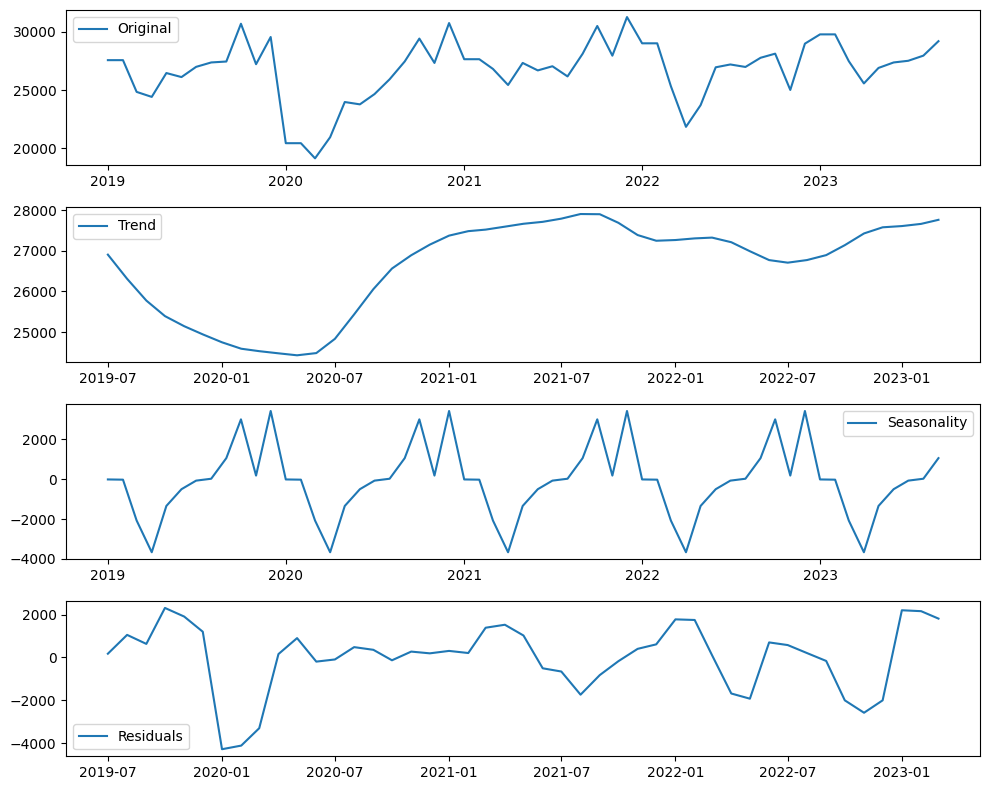
\includegraphics[width=0.6\textwidth]{Seasonal_analysis_offline.png}
    \caption{Offline Seasonal Analysis}
    \end{figure}

\end{frame}

\begin{frame}{Seasonal Analysis in Retail Sales}
\textbf{Online Trends:}
\begin{itemize}
    \item Monthly online sales show peaks likely due to promotional events.
    \item Long-term trend shows consistent growth in online sales.
    \item Seasonal cycles reflect the impact of holidays and sales events.
\end{itemize}


\begin{figure}
    \centering
    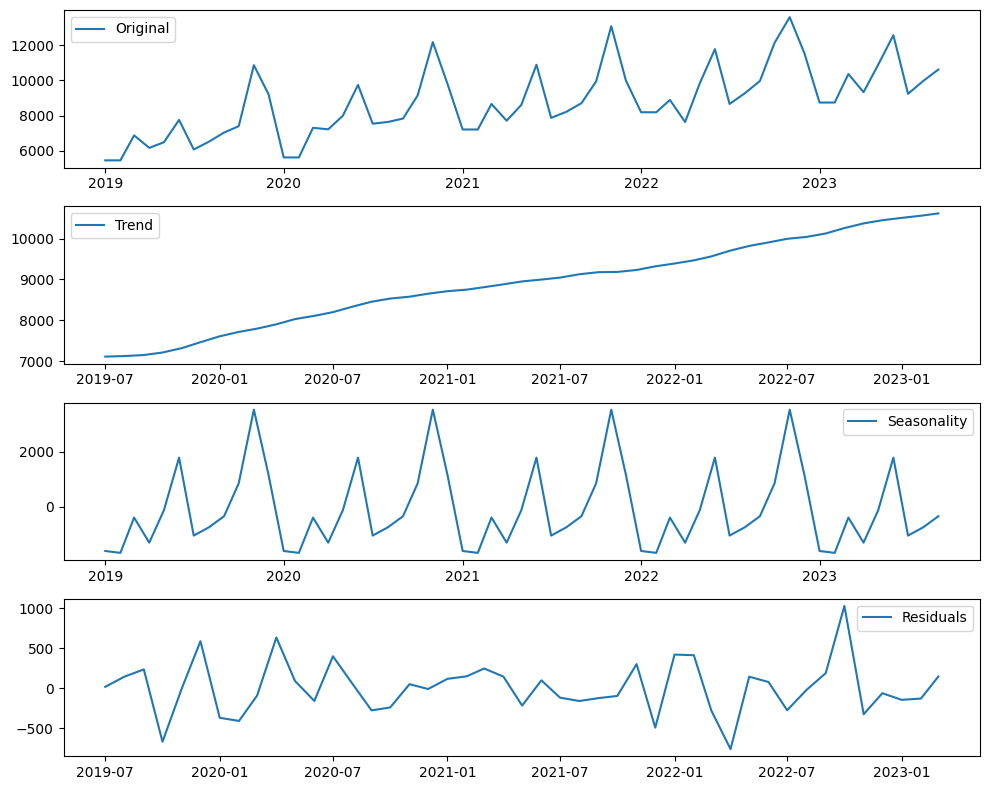
\includegraphics[width=0.6\textwidth]{Seasonal_analysis_online.png}
    \caption{Offline Seasonal Analysis}
    \end{figure}
    
\end{frame}






\begin{frame}{T test}
\begin{itemize}
    \item Conduct a t-test on the online monthly sales and offline monthly sales.
    \item The variances of the two sets of data are considered to be equal.
    \item There is a significant difference in the means of the two data samples.
\end{itemize}

\begin{table}[h]
\centering
\caption{Statistical Test Results}
\label{tab:stats-results}
\begin{tabular}{|l|S[table-format=-2.4]|}
\hline
\textbf{Test} & \textbf{Value} \\
\hline
Levene Statistics & 0.6410 \\
p-value (Levene) & 0.4250 \\
\hline
t Statistics & -41.4779 \\
p-value (t-test) & 1.066e-66 \\
\hline
\end{tabular}
\end{table}

\end{frame}

\begin{frame}{Regression analysis}
\begin{itemize}
    \item Statistically significant relationship.
    \item R-squared value of 0.108, indicating that online sales only modestly predict in-store sales.
    \item Contrary to expectations that online sales growth would weaken offline sales, both seem to be rising, possibly due to overall economic recovery post-pandemic.
\end{itemize}


\begin{figure}
    \centering
    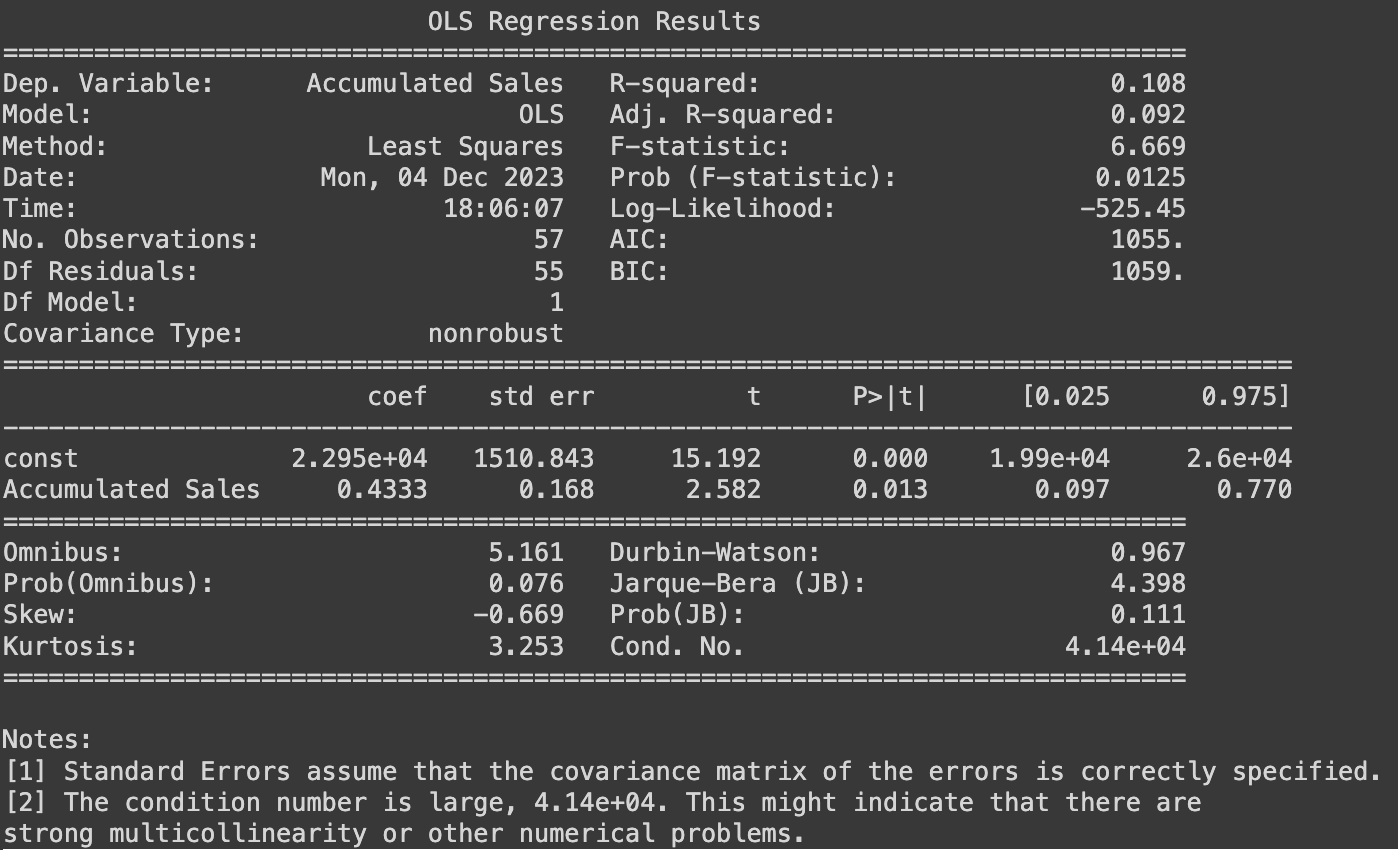
\includegraphics[width=0.55\textwidth]{Regression results.png}
    \caption{Regression analysis}
    \end{figure}


\end{frame}



\begin{frame}{Deseasonalized regression}
\begin{itemize}
    \item R-squared value of 0.162, indicating a stronger predictive power of online sales on in-store sales. 
    \item Suggesting a meaningful relationship between online and deseasonalized in-store sales.
  
\end{itemize}


\begin{figure}
    \centering
    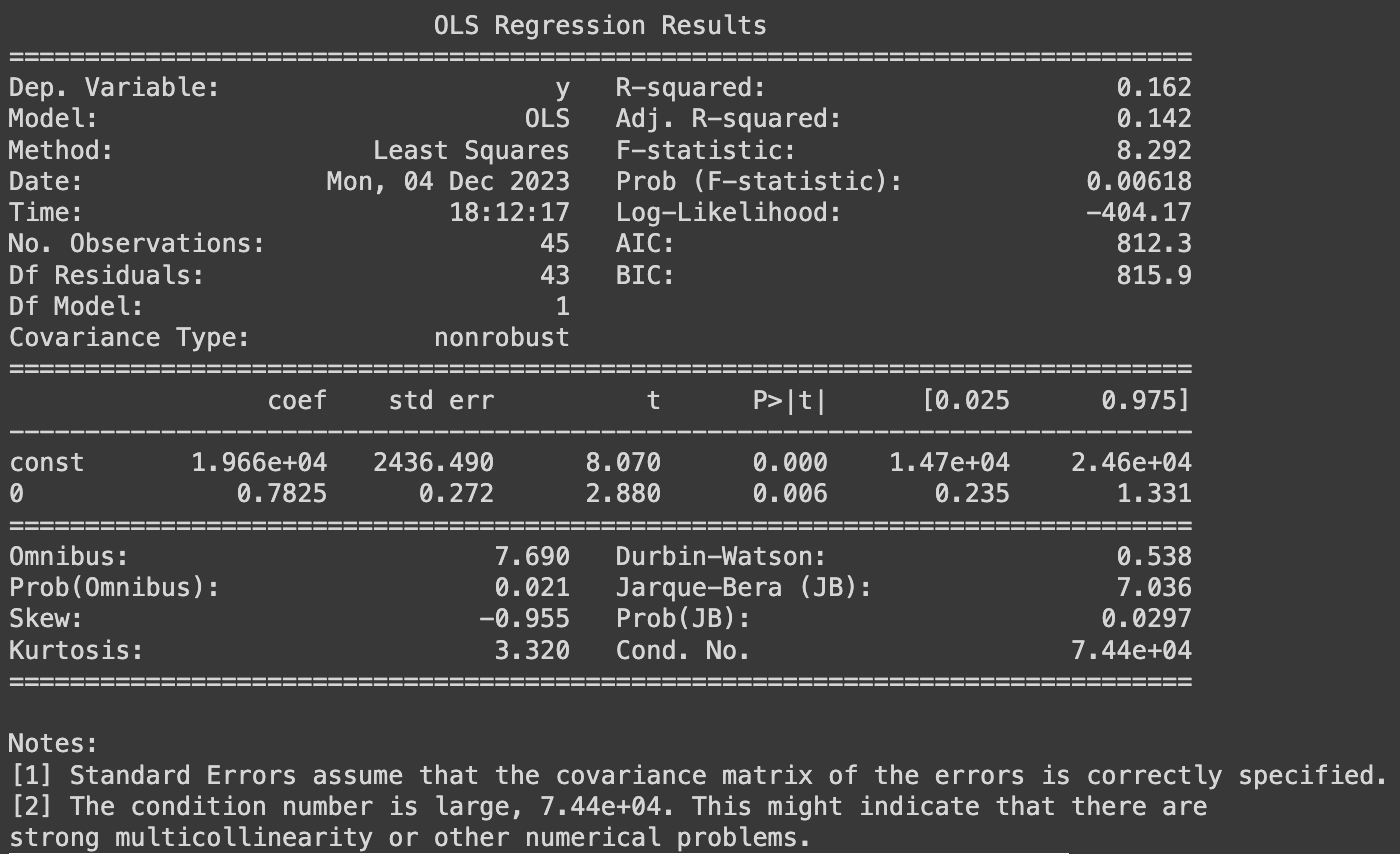
\includegraphics[width=0.55\textwidth]{Deseasonalized regression.png}
    \caption{Deseasonalized regression analysis}
    \end{figure}


\end{frame}

%---------------------------------------------------------

\begin{frame}{Conclusion}
\begin{itemize}
    \item  \textbf{Data-Driven Approach:} Utilized data from China's National Bureau of Statistics, analyzed via Python-based web scraping, covering the period from 2019 to 2023.
    \item \textbf{Consumer Shift to Digital:} Identified a significant consumer preference shift towards e-commerce platforms.
     \item \textbf{Impact of COVID-19:} Observed an acceleration in e-commerce adoption due to the pandemic, indicating lasting changes in consumer behavior.
     \item  \textbf{Seasonal Influence:} Detected the growing importance of seasonality in affecting both online and offline retail sales trends.
    \item \textbf{Future of Retail:} Contributed insights crucial for understanding and anticipating the future dynamics of retail in a digital-dominated era.
Impact of COVID-19: Observed an acceleration in e-commerce adoption due to the pandemic, indicating lasting changes in consumer behavior.
\end{itemize}




\end{frame}



\end{document}